\section{System Overview}
\textit{SnapSat} is an undergraduate project taken on by five students at the University of Sydney. The report will detail the Critical Design Review and specifications that were built to over the 12 week semester. The details of the subsystems and the system integration will be detailed here. The initial design point was for a three month mission at an orbit altitude of 350 kilometres and an inclination of 98\deg. However, this report will mainly detail the requirements for a 30km high-altitude balloon launch. Recommendations and upgrades to make this project viable for the initial design point will be made appropriately.


\subsection{Mission and Objectives}
The main mission of \textit{SnapSat} is to provide a platform to make space activities more accessible to the general public. The aim is to exploit popular social media and to allow the end user to post Twitter updates (Tweets) along with photographs of the Earth from the satellite. In order to do this, the cubesat needs a camera with sufficient resolution to see general country regions (and possible cities) along with a reliable communications connection to allow for fast data transfer at an orbit altitude of 350 kilometres. 
 
\subsection{Components and Subsystems}
On a primary level, for the deign on a high-altitude balloon, the main payload is the camera. Other basic requirements for the launch (power and communications) will be outlined in the following sections and discussed in detail later on in the report. An Attitude Determination and Control Subsystem (ADCS) was also tested and implemented as a proof-of-concept. The full structure was designed in-house and was a conventional laser-cut aluminium chassis. Details of the subsystems and the components chosen to meet each task are detailed in table~\ref{tab:components} below. The budget for the project was \$1000 provided by the School of Aerospace, Mechanical and Mechatronic Engineering at the University of Sydney. Components were selected based on their suitability for the project and for their cost. It was also important to take into consideration the working of other teams within the course. The communications structure chose relies on a `mother' satellite, through which all communications are managed. Components were selected to allow for this to work effectively. The purpose of having a mother sate little was to allow for an easy find after the high altitude balloon launch. 

\begin{table}[H]
   \centering
   \caption{Overview of component selection}
   \vspace{0.2cm}
   \label{tab:components}
   {\renewcommand{\arraystretch}{1.4}%
   \begin{tabular}{|>{\arraybackslash}m{3cm}|>{\arraybackslash}m{12cm}|}
         \hline
         \textbf{Subsystem} & \textbf{Chosen Components} \\ \hline\hline
         Structural & 	 - industrial grade Aluminium\newline
                         - laser cut, bent to shape and riveted together with M3 threaded rods to supports the Printed Circuit Boards (PCBs)\\\hline
         ADCS & 		 - air-core magnetorquers designed and made in house\newline
                         - OSRAM SFH203P photodiodes to track Sun location\newline
                         - Inertial Measurement Unit (IMU) to obtain gyroscopic data: Adafruit 10-DOF\\\hline
         EPS & - 9cm $\times$ 9cm solar 			panels\newline
                         - 2 $\times$ LiNiMnCo 26650 rechargeable cells\newline
                         - Adafruit voltage regulators\\\hline
         OBC/OBDH & - Microcontroller: Iduino DUE (Arduino DUE clone)\newline
                         - PCB $\times$ 4: power board, control systems and payload board, communications board, microcontroller board\\\hline
         TT\&C &
                         - RF 900 chip\newline
                         - duck antennae\newline
                         - Ublox 3.3V GPS\\\hline
         Thermal & 		 - passive coatings on cubesat chassis: kapton tape\\\hline
         Payload & 		 - camera: Arducam mini\\\hline  
   \end{tabular} } 
\end{table}

\subsection{System Integration}
Figure~\ref{fig:integration} below shows the schematic of how all the subsystems will work together and their communication protocol.
\begin{figure}[H]
    \centering
    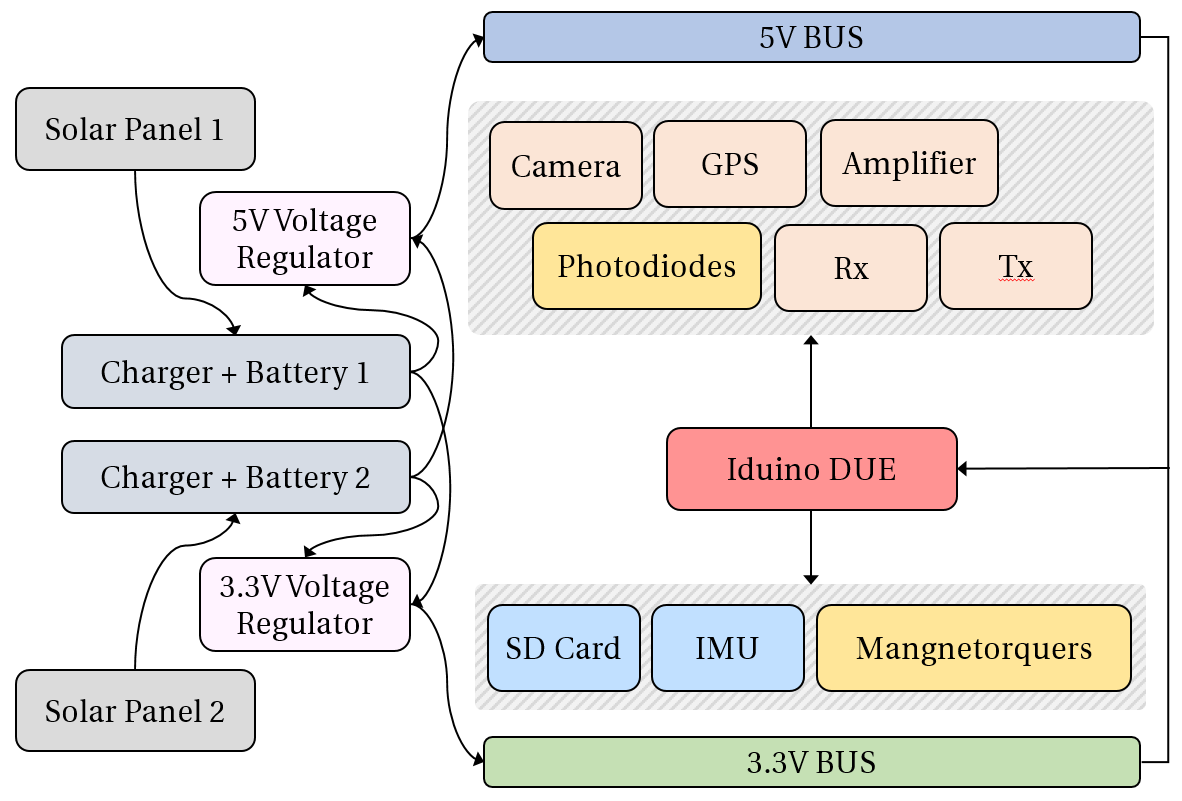
\includegraphics[width=0.75\linewidth]{./figures/integration}
    \caption{Full System Integration}
    \label{fig:integration}
\end{figure}
